%Empieza configuracion de capitulo
\setstretch{1.0}
\titleformat{\chapter}[block]{\Large\bfseries}{CHAPTER \Huge\thechapter\vspace{25 pt}}{0 pt}{\\\fontsize{26}{36}\selectfont}
\titlespacing{\chapter}{0 pt}{30 pt}{50 pt}[0 pt]
\titleformat{\section}{\Large\bfseries}{\thesection}{0 pt}{\hspace{30 pt}}
\titleformat{\subsection}{\large\bfseries}{\thesubsection}{0 pt}{\hspace{30 pt}}
\pagestyle{fancy}
\fancyhead[LO,LE]{\footnotesize\emph{\leftmark}}
\fancyhead[RO,RE]{\thepage}
\fancyfoot[CO,CE]{}
\setcounter{secnumdepth}{5}
%Termina configuracion de capitulo

\chapter{Theoretical Framework} \setstretch{1.5} %Regresa el interlineado a 1.5 \normalsize
\noindent

This chapter will describe some basic topics to help understand the
experiments described in chapters ahead and their justification.

\section{The need of parallel computing}
\noindent

Based on current technologies we have today (for example smartphones, tablets,
smart cars and more) the computer industry has achieved tremendous gain. 
Computer technology has been evolving like any other technology.
However, the progress of computer architectures has been much less
consistent. During the first 25 years of electronic computers \footnote{Since
1951 with the introduction of UNIVAC} the improvement in performance increased
about 25\% per year \cite{Hennessy}. 

It was at the beginning of the 1970s  when the world saw the emergence of the
microprocessor. Its appearance caused a major change in technology, which
allowed industry to improve scalability of integrated circuits. After the
introduction of the microprocessor, the improvement in performance per year on
computer architectures reached a 35\% \cite{Hennessy}.

However, advances in computer architecture were not the only responsible for
this great increase in performance. In particular, two significant changes made
the life of users easier. First, the invention of the C programing language, 
which caused a reduction in the development of assembly language programs, made
programs easier to read and to use. The C programing language gave the user the power to
handle memory and peripheral devices in a much more friendlier way. Second, the
creation of standardized and free  operating systems, such as UNIX and Linux.
These operating systems lowered the cost and risk of bringing out to the market
new products.

In the decade of 1980 the idea of making the microprocessor architecture faster
started to take form with the RISC (Reduced Instruction Set Computer)
architecture \cite{Hennessy}.  The RISC microprocessor is designed to perform a
smaller number of types of computer instructions so that it can operate at a
higher speed.  The RISC-based computers raised the performance bar. This
architecture principle in conjunction with the transistor size reduction
allowed to have much more computing power in less space it led to 16 years of
sustained growth in performance at an annual rate of over 50\%.

It was around the years 2003 to 2005 that a dramatic change seized the
semiconductor industry and the manufactures of processors. The increasing rate
of computing performance in processors, based simply on screwing up the clock
frequency, was not longer sustainable. The problem with increasing the
frequency in the microprocessor was that the heat in the chip also increased. In
fact, in 2004 Intel\textregistered\ canceled its high-performance uniprocessor
projects declaring that \textit{"the road to higher performance would be via
multiple processors per chip rather than via faster uniprocessors"} \cite{Hennessy}.

The answer of the industry to  meet Moore's law \footnote{The number of
transistors in a dense integrated circuit doubles approximately every two
years\cite{Mack}.}, was the shifting to real parallelism by doubling the number of
processors per chip die. This was the birth of the multicore era. 

With the multicore it emerged the need to change the paradigm in programing
languages. The programs that had been designed before this change were mostly a
sequence of instructions to calculate or control a system. The multicore
architecture brought the widespread of parallel programing. Parallel programing
is designed to provide faster execution of programs by executing independent
code section in parallel.

However, not all the problems can be solved using parallel programing
techniques. In order to use this approach the problem need to be represented as
a collection of simultaneously executing tasks. This is especially the case in
many areas of scientific, mathematical, and artificial intelligence
programming. After the birth of parallel computing, these technology
areas have evolved rapidly.

At the same time that parallel emerged, many other technologies were already
established: the emergence of the Internet, the World Wide Web, the cellphones,
and the laptops. According to \cite{Hennessy}, these technologies have led to
three different computing markets: desktop computing, servers and embedded. 

The problem studied in this work requires understanding of server and
embedded technologies.

\section{Servers Systems}
\noindent

The growth in the number of mobile personal computers coupled with the
popularity of cellphones. Such growth changed the role of servers to provide
scalable and reliable storage and computing services. The emergence of faster
Internet connections accelerated the demand of web-based services which caused
the transition of computing power from personal computers to servers.

However, the fact to provide storage and computing services to thousands of
users simultaneously implied a large responsibility. A failure on a server
system is by far more catastrophic than a failure of a single desktop computer
because servers must operate seven days per week, 24 hours per day. For this
reason, reliability is a key design parameter on server systems.

A second key feature on server systems is scalability. With the number of users
changing every minute the ability to scale up the computing capacity
in server is critical. A web sale site for sales must be able to respond every
request, as well
as during peak hours, for example during Christmas shoppings. A five minute
failure, might represent multimillion loses.

The third key design feature is throughput. Servers are designed for efficient
throughput \footnote{Throughput is a measure of how many units of information a
system can process in a given amount of time \cite{Dongxu}} in terms of
transactions per minute or Web pages served per second. From the user
perspective point of view this is the speed of response.

Due to the previously described design parameters the server technology has
evolved. The cloud era is dominating the computing and storage services.
According to \cite {Farhan} \textit{"Cloud computing is a set of resources and
services offered through the Internet"}. Cloud services are delivered from data
centers located around the world.  Cloud computing provides virtual resources
via the Internet. The best example of cloud computing is the streaming video of
video services. Nowadays, users can stream online videos  at any time, without the
need to storage the movies at home. All resources and infrastructure are
provided upon request. Scalability, reliability and throughput 
are guaranteed by computing service providers. 

\section{Embedded Systems}
\noindent

The birth of multicore architecture not only provides the servers with much
more computing power, but also breaks the paradigm of using low computing power
microprocessors for embedded platforms. Today it is possible to have more
computing power with less frequency. This change has allowed a rapid evolution
of computing and multimedia capabilities for embedded systems. The computers
technology has evolved in such a way that today there is more computing power
in a cellphone than all of NASA back in 1969 \cite{Michio}.

According to \cite{Hallinan} \textit{"An embedded system is a special-purpose
system in which the computer is completely encapsulated by the device it
controls"} Unlike a general-purpose computer, such as a personal computer, an
embedded system performs pre-defined tasks, usually with very specific
requirements. Examples of these are:microwaves, washing machines, printers, and
GPS (Global Positioning System) systems. These electronic gadgets started to
emerge more than 35 years ago \cite{Nur}.

The variety of embedded applications includes a wide spread of processing 
power and cost. They include 8-bit and 16-bit processors that may
cost a few cents, 32-bit microprocessors that execute 100 million instructions
per second and cost less than a few dollars, and high-end processors for the
newest video games or network switches that cost at least 100 dollars and can
execute one billion of instructions per second \cite{Hennessy}.

Since its origins, the RISC technology has been the default technology in
modern embedded architectures. Due to the fact that RISC
microprocessors are designed to execute a smaller number of types of 
instructions, the power consumption is smaller.

The increment in the complexity of new embedded applications started to
require more specialized integrated circuits that could support the microprocessor
to process tasks in parallel . Wireless networking cards, Digital Signal
Processors, I/O controls, peripherals (such as USB controllers) and analog
interfaces (including ADCs and DACs) became part of the requirements of an
embedded platform. Architecture designers realized that communication with 
these components decreased the performance and increased power consumption. For
that reason, during the last decade ti has been seen the emergence
of System on a Chip (SOC)  embedded platforms. 

The SoC is an integrated circuit with different processing components into a single chip.
Putting these components in the same integrated circuit the communication
latency and power consumption was reduced considerably. Since the beginning of 
SoC architectures the variety of gadgets using embedded platforms has
increased. Every year some new goals are pursued: for example, increment in
computing performance, cost,  size and power density reduction.

\section{Embedded Linux Systems}

Computers-based devices are everywhere. In office desktops, in our kitchens, in
living rooms, in microwave ovens, in regular ovens, in cellphones, in portable
digital music players, etc. 

A few years ago embedded systems were not very powerful, they executed
special-purpose, proprietary operating systems that were very different
from industry-standard ones. Today, embedded computers have more computing
capacity. 

Along with larger computing capacity it comes the capability to run a full-fledged operating
system, such as Linux. Using Linux for an embedded product
makes a lot of sense. The reasons are that it is a free operating system and it
has an easy user experience, such that the number of Linux users has increased 
rapidly. Linux has been one of the most sustainable projects in the history of computing. The fact that a
large community of developers finds novel ways to improve performance and fix
critical failures every day are the key to think that Linux could be the best
solution in terms of sustainability for embedded platforms.

According to \cite{Hallinan} there are multiple reasons why Linux is the best
choice for modern embedded platforms.

\begin{enumerate}
\item Linux supports a huge variety of applications and networking protocols.
Linux is scalable, from small consumer-oriented devices to large, heavy-iron,
carrier-class switches and routers.
\item Linux can be deployed without royalties required by traditional proprietary
embedded operating systems.
\item Linux has attracted a huge number of active developers, enabling rapid support
of new hardware architectures, platforms, and devices.
\item An increasing number of hardware and software vendors, including virtually all
of the top-tier manufacturers and ISVs.
\end{enumerate}

Due to these and other reasons, it is seen an accelerated adoption rate of
Linux in many common embedded platforms. With the birth of SoC systems the
use of complete operating systems was needed due to the requirement of handling
processes concurrency, memory management, and network connectivity.

Although the idea of using Linux as main operating system for embedded platform
was easy in reality it was not. With too many configure options and no standard
methodologies or templates to reuse the process to customize a Linux Operating
System for embedded platforms became a complex work for software engineers.
Every new embedded company create his own version (according to his needs
without any standards) with very low maintainability and robustness. In 2010
there was a change in the industry of embedded systems, the announce of a
project to solve these kind of problems: The Yocto project.

The Yocto Project is an open source collaboration project that provides
templates, tools and methods to help you create custom Linux-based systems for
embedded products regardless of the hardware architecture\cite{yocto-project}.
It was founded in 2010 as a collaboration among many hardware manufacturers,
open-source operating systems vendors, and electronics companies to bring some
order to the chaos of embedded Linux development \cite{Leppakoski}.

The Yocto project  is a  complete embedded Linux development environment with
tools, meta-data, and documentation. The free tools are easy to get started
with, powerful to work with (including emulation environments, debuggers, an
Application Toolkit Generator, etc.) and they allow projects to be carried
forward over time without causing you to loose optimizations and investments
made during the project's prototype phase. The Yocto Project fosters community
adoption of this open source technology allowing its users to focus on their
specific product features and development.

The Yocto Project through the Poky build tool provides an open source
development environment (figure~\ref{fig:3.1})  targeting the ARM, MIPS,
Power-PC and x86 architectures for a variety of platforms including x86-64 and
emulated ones.  You can use components from the Yocto Project to design,
develop, build, debug, simulate, and test the complete software stack using
Linux, the X Window System, GNOME Mobile-based application frameworks, and Qt
frameworks. 

\begin{figure}[H]
\centering
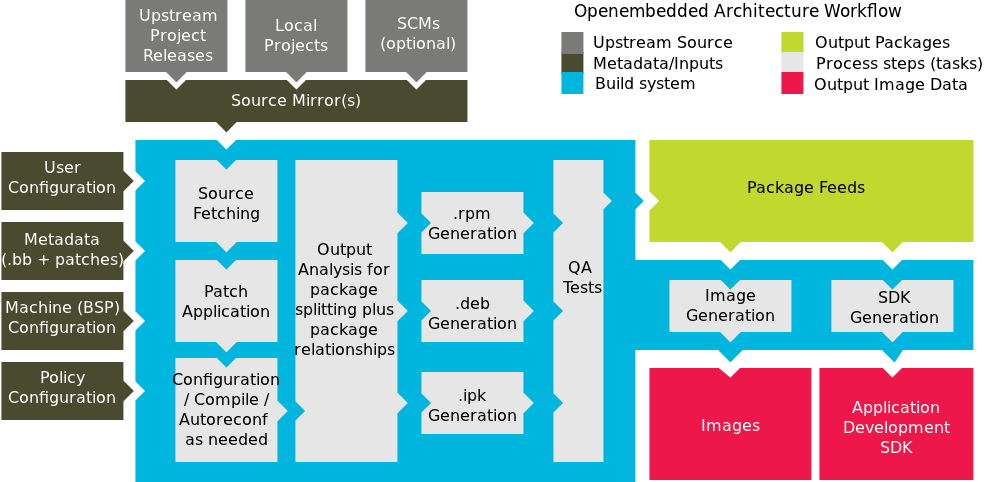
\includegraphics[width=1\textwidth]{images/yocto-environment.png}
\caption{The Yocto project development environment}
\label{fig:3.2}
\end{figure}

As we can see the Yocto project will play an important role in the IoT world.
If we want to develop a solution standard for multiple platforms we might adapt
it for the Yocto project. If we do this our solution will be deployable into
multiple IoT devices due to the bast amount of platforms ( sensors and
processing devices ) that use the Yocto project everyday.

\section{Ubiquitous Computing and IoT}
\noindent

The optimization of design parameters like cost, size, and power density
in combination with the increase in performance and connectivity
has made computing technology to evolve into ubiquitous computing.
According to Mark \cite{Mark}, ubiquitous computing is defined as \textit{"the method of
enhancing computer use by making many computers available throughout the
physical environment, but making them effectively invisible to the user"}. This
means that the computing power is available anywhere and at any time.

According to \cite{Nur}, nowadays ubiquitous computing is evolving into
advanced ubiquitous computing. An advanced ubiquitous computing is an extension
of an ubiquitous environment that improves connectivity between devices. The
main characteristics of this environment can be stated as follows: 

\begin{itemize}
\item A large number of heterogeneous devices.
\item Availability of new communication technology.
\end{itemize}

Ubiquitous computing includes devices such as notebook computers, tablets, smartphones
and wearable computers. Most of these devices operate under many different
operating systems. New communication technology 4G, 5G and the introduction of
IPv6 provides larger and faster data bandwidth than 3G.

One of the most accurate definitions of IoT is the one given by \cite{Bahga}
where it mentions that "Internet of Things refers to physical and virtual
objects that have unique identities and are connected to the internet to
facilitate intelligent applications.". IoT enables the interconnection, via the
Internet, of computing devices embedded in everyday use objects, enabling them
to send and receive data. The main difference of IoT systems with traditional
embedded systems is the Internet connectivity and less power consumption. IoT
systems must always be connected to the internet which require a lower power
consumption.

IoT computing is a new era of computing technology that explores in
collaboration with cloud computing the capability to have smart applications in
multiple scenarios. In the core of these technologies an invisible architecture
design was established, transparent to the user, but always there sustaining
the availability, scalability and reliability of systems, it was the
distributed systems architecture.

\section{Distributed Systems}
\noindent

We define a distributed system as one in which hardware or software components
located at networked computers communicate and coordinate their actions only by
passing messages \cite{Coulouris}. This simple definition covers the entire
range of systems in which networked computers can usefully be deployed.

Computers that are connected by a network may be spatially separated by any
distance. They may be on separate continents, in the same building, or in the
same room. The definition of distributed systems (given by \cite{Coulouris})
has the following significant characteristics:

\begin{enumerate}

\item \textbf{Concurrency:} 
In a network of computers, programs run concurrently. Programs share resources,
such as web pages, or files when necessary. The capacity of the system to handle
shared resources can be increased by adding more resources (for example.
computers or memory) to the network.

\item \textbf{No global clock:}
When programs need to cooperate, they coordinate their actions
by exchanging messages. Close coordination often depends on a shared idea of
the time at which the programs actions occur. But it turns out that there are
limits to the accuracy with which the computers in a network can synchronize
their clocks there is no single global notion of the correct time. This is a
direct consequence of the fact that the only communication is by sending
messages through a network.

\item \textbf{Independent failures:}
All computer systems can fail, and it is the
responsibility of system designers to plan for the consequences of possible
failures. Distributed systems can fail in new ways. Faults in the network
result in the isolation of the computers that are connected to it, but that
doesn't mean that they stop running. In fact, the programs on them may not be
able to detect whether the network has failed or has become unusually slow.
Similarly, the failure of a computer, or the unexpected termination of a
program somewhere in the system (a crash), is not immediately made known to the
other components with which it communicates. Each component of the system can
fail independently, leaving the others still running.

\end{enumerate}

Each one of these characteristics is also present in a modern IoT system. 
Figure \ref{fig:3.1} represents an IoT system showing its distributed systems
characteristics. 

\begin{figure}[H]
\centering
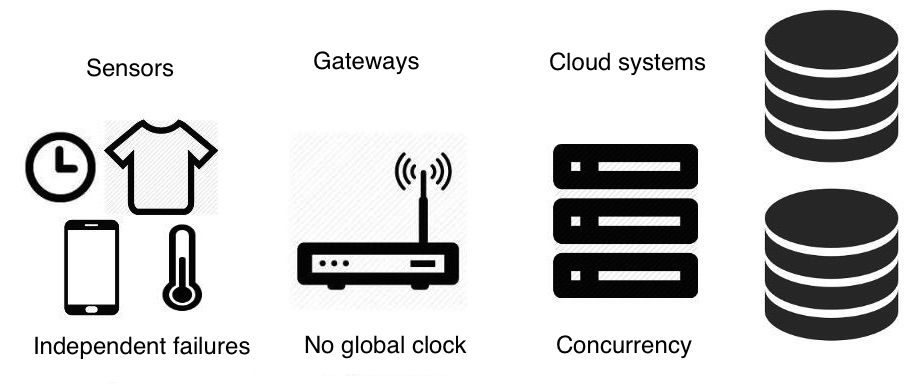
\includegraphics[width=1\textwidth]{images/IoT_distributed.jpeg}
\caption{IoT system as a distributed system}
\label{fig:3.1}
\end{figure}


\begin{enumerate}
\item \textbf{Concurrency:}
In an IoT system there are multiple systems trying to use the same resource.
For example, all IoT devices are trying to access the same data base or
the same access point. All of them are competing for similar resources, a
good IoT design needs to schedule the use of limited resources in an efficient
way.

\item \textbf{No global clock:}
None of the systems in an IoT network (either sensors or processing devices)
have the same clock. They have to use a message-based mechanism to communicate
with each other. 

\item \textbf{Independent failures}
In a regular IoT network multiple systems could fail (either sensors,
processing devices, or one of the data centers). Despite of the failures others
components should keep working without any problem.

All these characteristics enforce the idea that the nature of an IoT system is
being treated as a distributed system. With this idea it is simpler to adapt
solutions of distributed systems into IoT distributed systems.

\end{enumerate}

\section{Message-Passing Interface Library}
\noindent

The Message-Passing Interface (MPI) is a message-passing library interface
specification. MPI addresses primarily the message-passing parallel programming
model, in which data is moved from the address space of one process to that of
another process through cooperative operations on each process.

MPI is not a language, and all MPI operations are expressed as functions,
subroutines, or methods, according to the appropriate language bindings which,
for C and FORTRAN, are part of the MPI standard. The standard has been defined
through an open process by a community of parallel computing vendors, computer
scientists, and application developers.

Despite all the advantages that MPI has it is not widely used in embedded
systems (due to the fact that these abstraction layers require extensive
system resources with comprehensive operating systems support, which may not be
available to an embedded platform) but as we have seen this is now possible. We
do have a powerful ultra-low-voltage microprocessor platform
\cite{minnowboard} and we do have robust distributed operating systems running on
those platforms. The missing part now is to set up the message passing library
interface on the top of all the system. 

Recent researches \cite{Saldana} \cite{Gallego} \cite{McMahon} describe
proof-of-concept MPI implementations targeting embedded systems, showing an
increasing interest in the topic. However none of theme has been implemented in
the current embedded Linux operating systems (like the ones generated with
Yocto project\cite{yocto-project}) nor the standard Linux (like
Fedora\cite{fedora}).

After a quick review on the current operating systems we found that the only
one missing the MPI implementation was actually the Yocto project.


\begin{center}
\begin{tabular}{ | l | r |}
    \hline
    Operating System & MPI library  \\ \hline
    Fedoras & Implemented  \\ \hline
    Clear Linux for Intel Architecture & Implemented  \\ \hline
    OS generated with Yocto project & Not Implemented  \\ \hline
\end{tabular}
\captionof{table}{Linux OS supported MPI implementation on MinnowBoard MAX}
\label{tab:4.2}
\end{center}


\section{Performance and Power Efficiency}

\noindent

The meaning of performance may be different according to the application.
The user of a desktop computer may say a computer is faster when a program runs in less
time, while an Amazon.com administrator may say a computer is faster when it
completes more transactions per hour. The computer user is interested in 
reducing response time (the time between the start and the completion of an 
event) \cite{Hennessy} also referred to as execution time. The administrator of a large data 
processing center may be interested in increasing throughput (the total amount 
of work done in a given time.) \cite{Hennessy}. 

According to \cite{Hennessy} in comparing design alternatives, we often want to
relate the performance of two different computers, say, X and Y. The phrase ''X
is faster than Y'' is used here to mean that the response time or execution
time is lower on X than on Y for the given task. In particular, ''X is n times
faster than ''  will mean \ref{eq:2}:

\begin{equation}\label{eq:2}
n = \frac{Execution time x}{Execution time y}
\end{equation}

Since execution time is the reciprocal of performance, the following
relationship holds in formula \ref{eq:3}:

\begin{equation}\label{eq:3}
n = \frac{Execution time x}{Execution time y} = \frac{\frac{1}{Performance
x}}{\frac{1}{Performance y}} = \frac{Performnace x}{Performance y}
\end{equation}

Another metric to considerate is the throughput. According to \cite{Hennessy}
\textit{"the throughput of X is 1.3 times higher than Y signifies that the
number of tasks completed per unit time on computer X is 1.3 times the number
completed on Y"} . Unfortunately, time is not always the metric quoted in
comparing the performance of computers. The only consistent and reliable
measure of performance is the execution time of real programs. 

The most straightforward definition of execution time is given by
\cite{Hennessy} \textit{"it is called wall-clock time, response time, or elapsed
time, which is the latency to complete a task, including disk accesses, memory
accesses, input/output activities, operating system over head everything"}.
Even in current multi processors world this is transparent for the users,  the
response time seen by the user is the elapsed time of the program, not the CPU
time.

But in parallel programing the performance metric is measure in a different
way.  With the current compute power of compute devices is possible to create a
cluster of computers. All of the inter-connected in a network that provides the
maximum level of performance with the less amount of power consumption. This
characteristic is determined by the power efficiency of the network. The power
efficiency is quantified by performance per watt \cite{Jun}.

The critical part is to determine the breaking point where is better to send
the data to the cloud data centers. How many systems is the maximum that these
kind of network could support and still being a good option in terms of energy
efficiency.

The development of metrics to evaluate energy efficiency on the basis of
performance and power models is described in \cite{Dong}. According to
\cite{Dong} the formula for computing the theoretical maximum speedup (or
performance) achievable through parallelization is \ref{eq:4}.

\begin{equation}\label{eq:4}
Perf = \frac{1}{(1 - f) + \frac{f}{n}}
\end{equation}

Where \textit{n} is the number of processors,  \textit{f} is the fraction of
computation that programmers can parallelize  ( form 0 to 1 ) . To model the
power consumption for a \textit{P} many-core processor, \cite{Dong} introduce a
new variable, \textit{k}, to represent the fraction of power the processor
consumes in idle state \ref{eq:5}. 

\begin{equation}\label{eq:5}
\frac{Perf}{W} = \frac{1}{(1 + (n -1 ) k (1 - f))}
\end{equation}

In \cite{Dong} their analysis clearly demonstrates that a symmetric many-core
processor can easily  lose its energy efficiency as the number of cores
increases. To achieve the  best possible energy efficiency, their  work
suggests a many-core alternative, featuring many small, energy-efficient cores
integrated with a full-blown processor. They also show that by knowing the
amount of parallelism available in an application prior to execution, is
possible to  find the optimal number of active cores for maximizing performance
for a given cooling capacity and energy in a system.

\section{Benchmarks}

In computer science a benchmark is a test to measure the performance of
multiple applications over the same standard way. The best choice of benchmarks
to measure performance are real applications. Due to the complexity of the
current applications the software engineers are making small versions of them
to be used as benchmarks. According to \cite{Hennessy} there are three kind of
them: 

\begin{itemize}
\item kernels, which are small, key pieces of real applications.
\item Toy programs, which are 100-line programs from beginning programming
assignments.
\item Synthetic benchmarks, which are fake programs invented to try to match the
profile and behavior of real applications.
\end{itemize}

One of the most successful attempts to create standardized benchmark
application suites has been the SPEC (Standard Performance Evaluation
Corporation), which had its roots in the late 1980s efforts to deliver better
benchmarks for workstations\cite{Hennessy}. All the SPEC benchmark suites and
their results are found at www.spec.org.

In terms of parallel and distributed computing (MPI) there are already numerous
MPI benchmark suites available , such as Mpptest \cite{Gropp}, MP-Bench
\cite{Calderon} and  SKaMPI \cite{Hoefler} are examples of them. Many of give
timing results for message passing routines. This is useful for performance
modelling and analysis of parallel programs, as well as for understanding the
performance of parallel machines. Based on the results in \cite{Grove} we
decided to use MPIbench as our default benchmark testing framework. MPIbench is
a benchmark that allows to evaluate the performance of MPI on MPP's and cluster
of workstations. MPIbench tests different MPI calls.

\subsection{MPIbench}
\noindent

The benchmarks we are going to run are the MPIbench (or MPbench) version 4
\cite{mpibench}.This is a program to measure the performance of some critical
MPI functions. By critical we mean that the behavior of these functions can
dominate the run time of a distributed application.

MPIBench currently tests eight different MPI calls. The following functions are
measured:

\begin{itemize}
    \item Bandwidth (BB/second)
    \item Gap Time (time to launch a message and continue) (Us)
    \item Roundtrip or 2 * Latency (transactions/second)
    \item Asynchronous Bidirectional bandwidth (KB/second)
    \item Broadcast (KB/second)
    \item Sum reduction (KB/second)
    \item All-reduce (KB/second)
    \item AlltoAll (KB/second)
\end{itemize}


All tests are timed in the following manner.

\begin{itemize}
    \item Set up the test.
    \item Start the timer.
    \item Loop of operations over the message size as a power of two and the
iteration count.
    \item Verify that those operations have completed.
    \item Stop the timer.
    \item Compute the appropriate metric
\end{itemize}

By default, MPIBench measures messages from 4 bytes to 216 bytes, in powers of
two for 100 iterations. Each test is run a single time before testing to allow
for cache setup and routing. The cache is then flushed before each repetition
and before each new message size is tested. The cache is not flushed however
between iterations on the same message size, which are averaged

We will describe each one of the tests in order to understand the experiments.


\subsubsection{Bandwidth}

MPIBench measures bandwidth with a doubly nested loop. The outer loop varies the
message size, and the inner loop measures the send operation over the
iteration count. After the iteration count is reached, the slave process
acknowledges the data it has received by sending a four byte message back to
the master. The master's pseudo code for this test is as follows:

\begin{minipage}{\textwidth}
\end{minipage}

\begin{minipage}{\linewidth}
\begin{lstlisting}[frame=single,numbers=left]
do over all message sizes 
    start timer
    do over iteration count 
        send(message size) 
        recv (4)
    stop timer
\end{lstlisting}
\end{minipage}

The slaves' pseudo code is as follows:

\begin{minipage}{\textwidth}
\end{minipage}

\begin{minipage}{\textwidth}
\begin{lstlisting}[frame=single,numbers=left]
do over all message sizes 
    start timer
    do over iteration count 
        recv(message size) 
        send(4)
    stop timer
\end{lstlisting}
 \end{minipage}

\subsubsection{Bidirectional Bandwidth}

MPIBench measures bidirectional bandwidth with a doubly nested loop. The outer
loop varies the message size, and the inner loop measures the send operation
over the iteration count. Both processes execute a non-blocking receive, then a
non-blocking send, and then a wait for each iteration. The next iteration is
prevented from proceeding until the previous one is finished by the MPLWaitall0
call, which will not allow execution to continue until both messages have been
completed.

The code for this test is as follows:
 
\begin{minipage}{\textwidth}
\end{minipage}

\begin{minipage}{\textwidth}
\begin{lstlisting}[frame=single,numbers=left]
 do over all message sizes
    start timer
    do over iteration count
        immediate (nonblocking) receive(message size)
        immediate (nonblocking) send(message size)
        wait until messages on both ends have been received
    stop timer
\end{lstlisting}
\end{minipage}

\subsubsection{Roundtrip}

Roundtrip times are measured in much the same way as bandwidth, except that,
the slave process, after receiving the message, echoes it back to the master.
This benchmark is often referred to as ping-pong. Here our metric is
transactions per second, which is a common metric for database and server
applications. No acknowledgment is needed with this test as it is implicit
given its semantics.

The master's pseudo code for this test is as follows:

\begin{minipage}{\textwidth}
\end{minipage}

\begin{minipage}{\textwidth}
\begin{lstlisting}[frame=single,numbers=left]
  do over all message sizes 
    start timer
    do over iteration count
        send(message size)
        recv(message size) 
        stop timer
\end{lstlisting}
\end{minipage}

The slaves' pseudo code is as follows:

\begin{minipage}{\textwidth}
\end{minipage}

\begin{minipage}{\textwidth}
\begin{lstlisting}[frame=single,numbers=left]
do over all message sizes 
    start timer
    do over iteration count
        recv(message size)
        send(message size)
    stop timer
\end{lstlisting}
\end{minipage}

\subsubsection{Application Latency}

Application latency is something relatively unique to MPBench. This benchmark
can properly be described as one that measures the time for an application
to issue a send and continue computing. This benchmark is the same as
bandwidth except that we do not acknowledge the data and we report our
results in units of time.

The master's pseudo code for this test is as follows:

\begin{minipage}{\textwidth}
\end{minipage}

\begin{minipage}{\textwidth}
\begin{lstlisting}[frame=single,numbers=left]
do over all message sizes 
    start timer
    do over iteration count 
        send(message size) 
    stop timer
\end{lstlisting}    
\end{minipage}

The slaves' pseudo code is as follows:

\begin{minipage}{\textwidth}
\end{minipage}

\begin{minipage}{\textwidth}
\begin{lstlisting}[frame=single,numbers=left]
   do over all message sizes 
        start timer
        do over iteration count 
            recv(message size) 
        stop timer
\end{lstlisting}
\end{minipage}

\subsubsection{Broadcast and Reduce}

Both of these benchmarks return the number of megabytes per second computed
from the iteration count and the length argument given to function call.

Here is the pseudo code for both the master and the slave:

\begin{minipage}{\textwidth}
\end{minipage}

\begin{minipage}{\textwidth}
\begin{lstlisting}[frame=single,numbers=left]
   do over all message sizes 
        start timer
        do over iteration count
            reduce or broadcast(message size)
        stop timer
\end{lstlisting}
\end{minipage}

\subsubsection{AllReduce}

AllReduce is a derivative of an all-to-all communication, where every
process has data for every other. While this operation could easily be
implemented with a reduce followed by a broadcast, that would be highly
inefficient for large message sizes. 

Here is the pseudo code for both the master and the slave:

\begin{minipage}{\textwidth}
\end{minipage}

\begin{minipage}{\textwidth}
\begin{lstlisting}[frame=single,numbers=left]
    do over all message sizes 
        start timer
        do over iteration count 
            allreduce(message size) 
        stop timer
\end{lstlisting}
\end{minipage}

\subsubsection{All-to-all}

MPBench measures a kind of round-robin communication among multiple
processes. The outer loop varies the message size, and the inner loop
measures the send operation over the iteration count. Each process sends a
message of the size of the total message size divided by the number of
processes to every other process.

The code for this test is as follows:

\begin{minipage}{\textwidth}
\end{minipage}

\begin{minipage}{\textwidth}
\begin{lstlisting}[frame=single,numbers=left]
    do over all message sizes 
        start timer
        do over iteration count 
            all-to-all(message size)
        stop timer
\end{lstlisting}
\end{minipage}

\clearpage
